\documentclass{article}

% Language setting
% Replace `english' with e.g. `spanish' to change the document language
\usepackage[french]{babel}
\usepackage[fleqn]{amsmath} % Aligner les équations à gauche


% Set page size and margins
% Replace `letterpaper' with`a4paper' for UK/EU standard size
\usepackage[letterpaper,top=2cm,bottom=2cm,left=3cm,right=3cm,marginparwidth=1.75cm]{geometry}

% Useful packages

\usepackage{amsmath}
\usepackage{graphicx}
\usepackage{subcaption}
\usepackage[colorlinks=true, allcolors=blue]{hyperref}

\title{Numerical tours report}
\author{Grégoire Béchade}
% \date{7 février 2024}

\begin{document}
\maketitle



\section{Tour 1}

I have decided to work with the following distribution (\ref{fig:2distrib}) to study the optimal transport on a circular distribution. 




\begin{figure}[h]
  \centering
  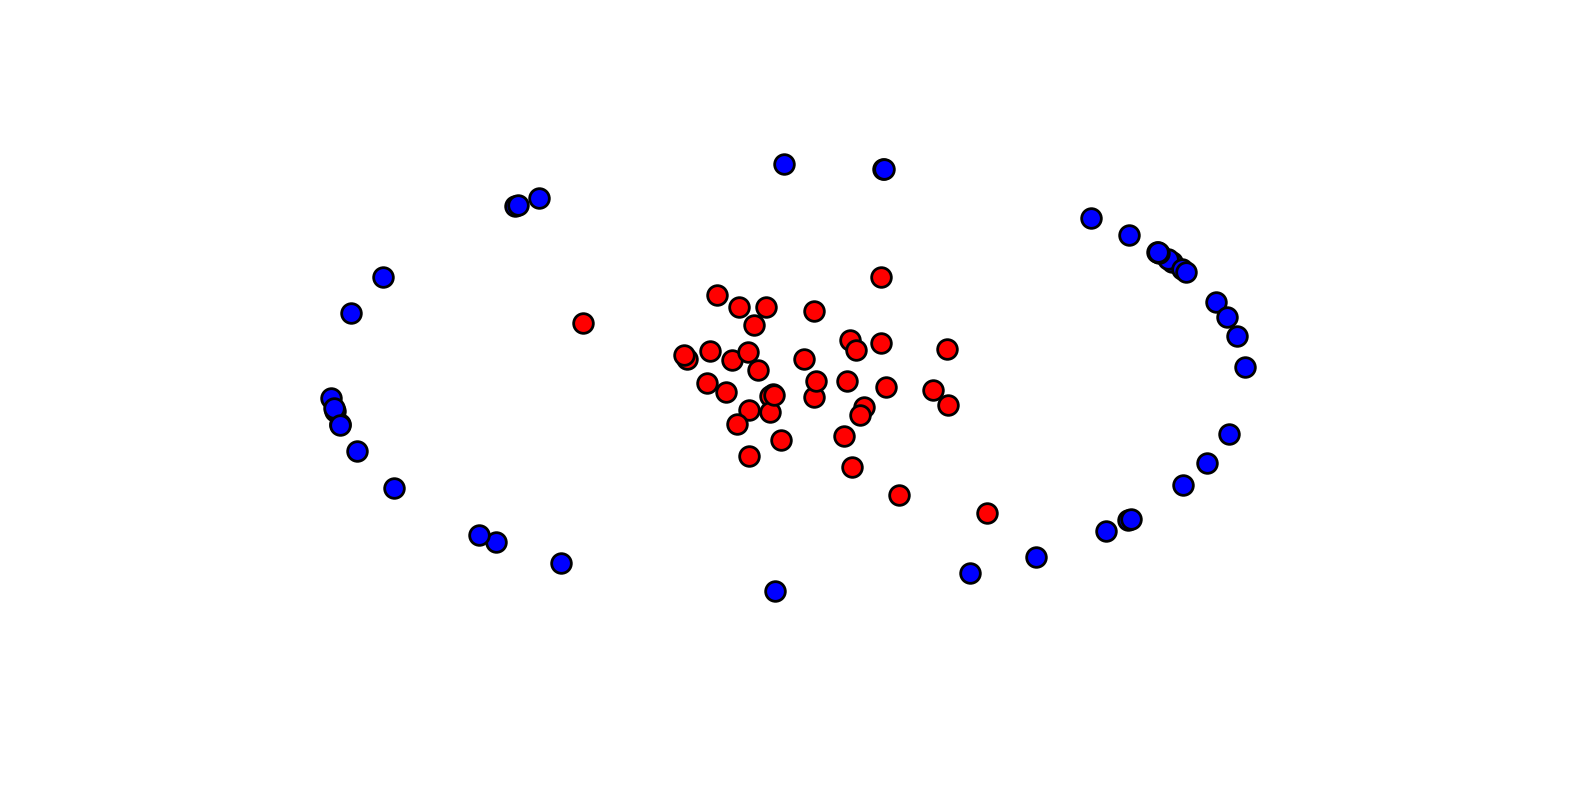
\includegraphics[width=0.3\textwidth]{images/distrib.png}
    \caption{The two weighted distributions}
  \label{fig:2distrib}
\end{figure}

When solving the Kantorovich problem, we observe what was expected: the mass of a dirac is transported toward its nearest neighbourghs (\ref{fig:transport}).
\begin{figure}[h]
  \centering
  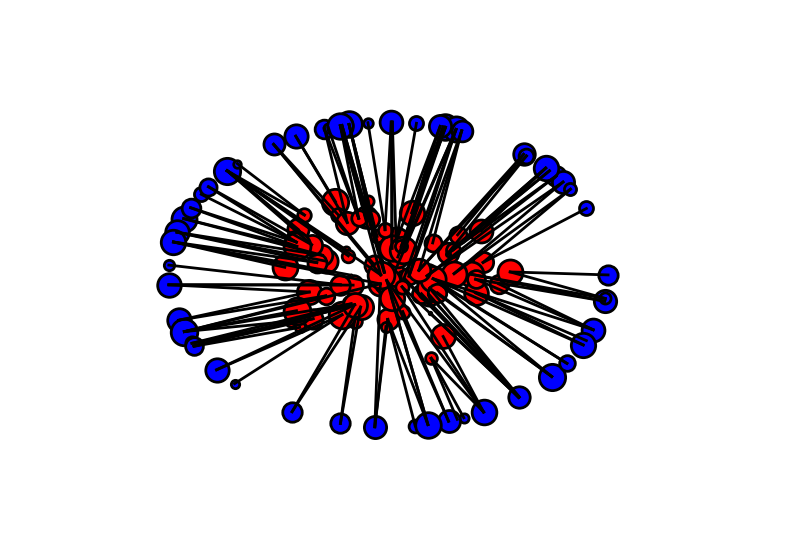
\includegraphics[width=0.3\textwidth]{images/close.png}
    \caption{Kantorovich transport}
  \label{fig:transport}
\end{figure} 

When solving the same probmlem but with $n=m$, I have observed as expected that the solution is a permutation matrix (\ref{fig:permutation}). 
therefore, using Kantorovich relaxation enables to use the exact solution of the equivalent Monge's problem.  

\begin{figure}[h]
  \centering
  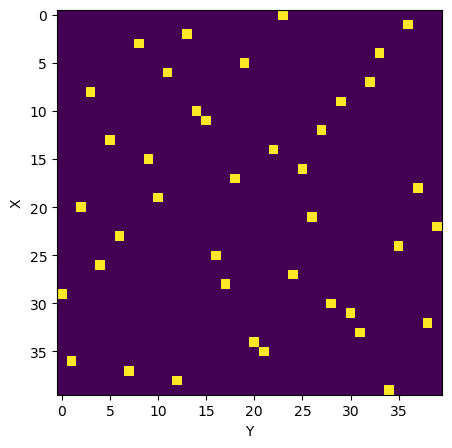
\includegraphics[width=0.2\textwidth]{images/permutation_matrix.png}
  \caption{Permutation matrix of the solution of the Kantorovich problem}
  \label{fig:permutation}
\end{figure}



\end{document}

